\documentclass[logo,reportComp]{thesis}
\usepackage[cpp]{mypackage}

\title{分布式系统作业六}
\subtitle{}
\school{数据科学与计算机学院}
\author{陈鸿峥}
\classname{17大数据与人工智能}
\stunum{17341015}
\headercontext{分布式系统作业}

\begin{document}

\maketitle

\begin{question}
对以下每个应用程序,你认为最多一次语义和最少一次语义哪个更好?
\begin{itemize}
\item [(a)] 从文件服务器上读写文件;
\item [(b)] 编译一个程序;
\item [(c)] 远程银行
\end{itemize}
\end{question}
\begin{answer}
\begin{itemize}
	\item [(a)] 最少一次(at least once)最好,因为可以重复多次尝试读写文件,失败后继续尝试
	\item [(b)] 最少一次语义。同样可以重复多次尝试编译程序。
	\item [(c)] 最多一次语义。为避免银行资金出现紊乱,服务器保证操作至多执行一次,当出现故障时最好进行人工干预(比如到银行柜台办理手续)。
\end{itemize}
\end{answer}

\begin{question}
简述Flooding、 PAXOS、 RAFT、 PBFT、 PoW的使用场景?
\end{question}
\begin{answer}
\begin{itemize}
	\item Flooding:能够准确检测到失效,但是通讯量非常大,因为两两之间都要进行消息传递,泛洪共识在现实生活中已经用得很少了,更多是采用下面的共识协议\cite{bib:flooding}。
	\item PAXOS:能够最终检测到失效,但是非常复杂,非常难实施;Google的NewSQL数据库Spanner\cite{bib:spanner}就是基于PAXOS搭的。
	\item RAFT:非拜占庭故障下达成共识的强一致性协议,也能最终检测到实现,但比PAXOS要好理解及好实现;在各种数据库及分布式系统中被广泛使用\cite{bib:raft}。
	\item PBFT:可以实现拜占庭容错,在区块链中会使用。其中的Leader选举是采用一种轮询的方式\cite{bib:pbft}。
	\item PoW:现在的区块链用得最多,通过工作量/算力达成共识。PoW即确认工作端做过一定量工作的证明。比如在比特币系统\cite{bib:bitcoin}中,大约每10分钟进行一轮算力比赛,获胜者将获得一次记账的权力,并向其他节点同步新增账本信息。
\end{itemize}
\end{answer}
% * 失效容错
% 	* 准确检测失效:flooding
% 	* 最终检测失效
% 		* PAXOS
% 		* RAFT
% 		* ZAB
% * 拜占庭容错
% 	* BFT
% 	* PBFT
% 	* POW

\begin{question}
任意选择一种编程语言实现的RAFT程序,运行该程序并测试记录结果。
\begin{itemize}
	\item \url{https://github.com/logcabin/logcabin}
	\item \url{https://github.com/streed/simpleRaft}
\end{itemize}
\end{question}
\begin{answer}
我使用了LogCabin进行测试。
LogCabin是一个基于raft的分布式存储系统,提供可靠、高度冗余、一致性的存储。

按照官方教程,需要先在Ubuntu系统安装scons、protobuf和crypto++,然后调用scons进行编译。

编译完成后,开启3个服务器端组成一个集群,服务器配置如下:
\begin{lstlisting}
// File logcabin-1.conf
serverId = 1
listenAddresses = 127.0.0.1:5254

// File logcabin-2.conf
serverId = 2
listenAddresses = 127.0.0.1:5255

// File logcabin-3.conf
serverId = 3
listenAddresses = 127.0.0.1:5256
\end{lstlisting}
然后通过以下指令,开启服务器工作(注意要开启3个不同的命令行)
\begin{lstlisting}[language=bash]
build/LogCabin --config logcabin-1.conf --bootstrap
build/LogCabin --config logcabin-1.conf # first terminal
build/LogCabin --config logcabin-2.conf # second terminal
build/LogCabin --config logcabin-3.conf # third terminal
\end{lstlisting}
然后开启第4个命令行,执行下列指令,将3个服务器捆绑为一个集群(cluster)。
\begin{lstlisting}[language=bash]
ALLSERVERS=127.0.0.1:5254,127.0.0.1:5255,127.0.0.1:5256
build/Examples/Reconfigure --cluster=$ALLSERVERS set 127.0.0.1:5254 127.0.0.1:5255 127.0.0.1:5256
\end{lstlisting}
会得到如下配置成功信息
\begin{figure}[H]
\centering
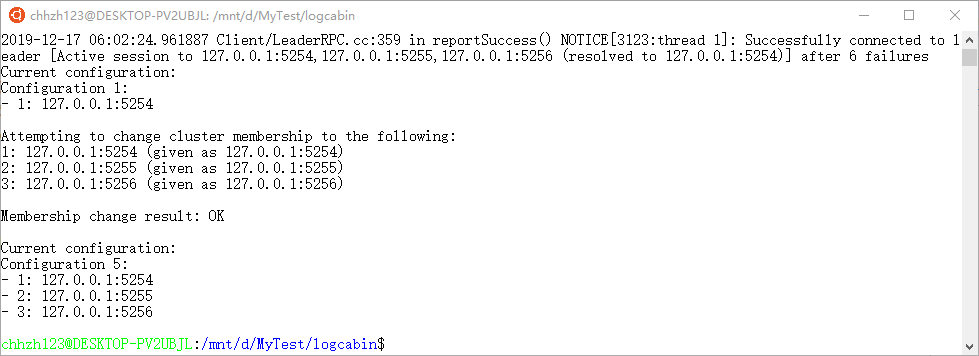
\includegraphics[width=\linewidth]{fig/config.png}
\end{figure}
同时在服务器端上也会显示新成员加入信息
\begin{figure}[H]
\centering
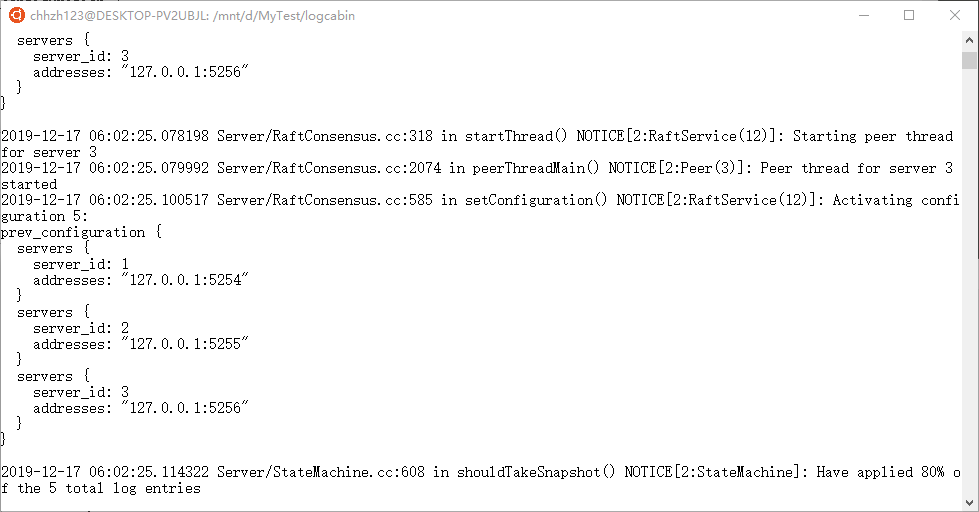
\includegraphics[width=\linewidth]{fig/server.png}
\end{figure}

执行过程截图如下所示,有1个Leader,其余2个为Follower。
\begin{figure}[H]
\centering
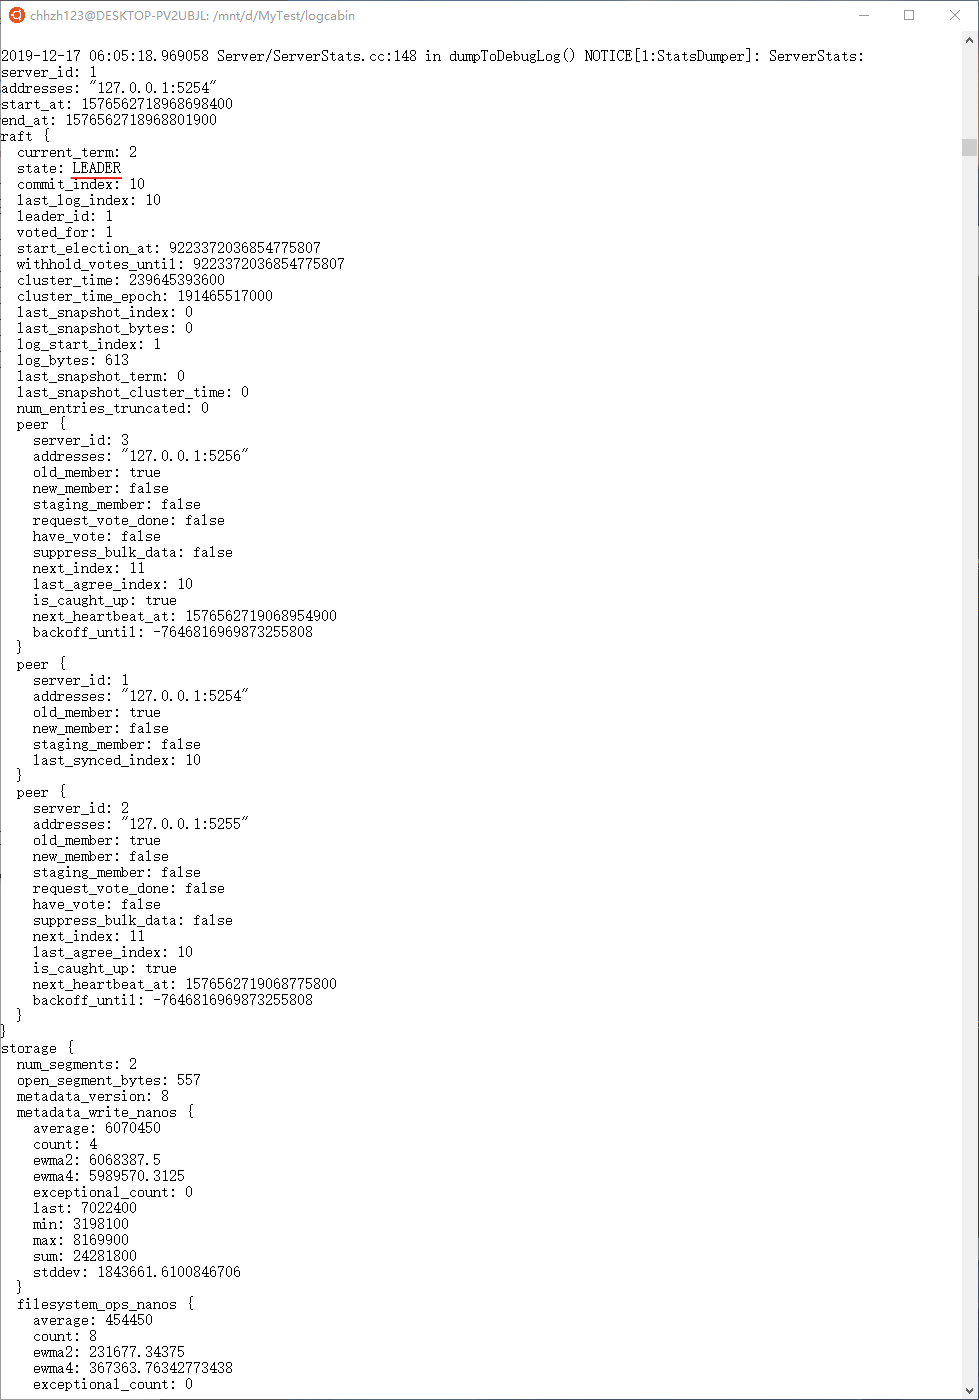
\includegraphics[width=\linewidth]{fig/leader.png}
\end{figure}
\begin{figure}[H]
\centering
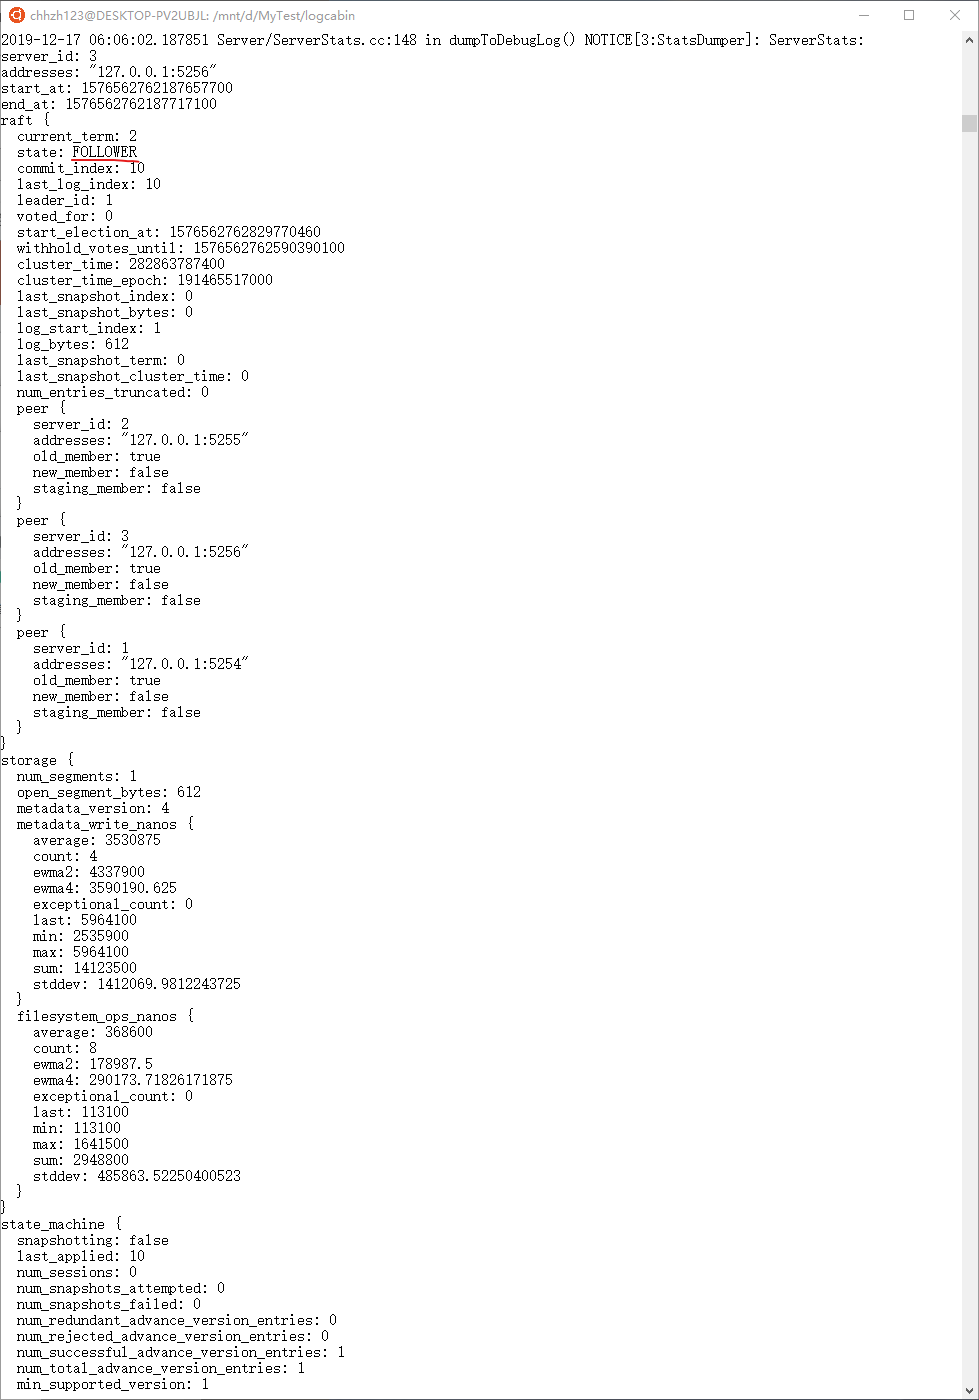
\includegraphics[width=\linewidth]{fig/follower.png}
\end{figure}

接下来测试其文件功能,采用下述执行进行简单的文件操作。
\begin{lstlisting}[language=bash]
build/Examples/TreeOps --cluster=$ALLSERVERS mkdir /test
echo -n hello | build/Examples/TreeOps --cluster=$ALLSERVERS write /world
build/Examples/TreeOps --cluster=$ALLSERVERS dump
\end{lstlisting}
最终可以看到test目录和world文件都成功生成。
\begin{figure}[H]
\centering
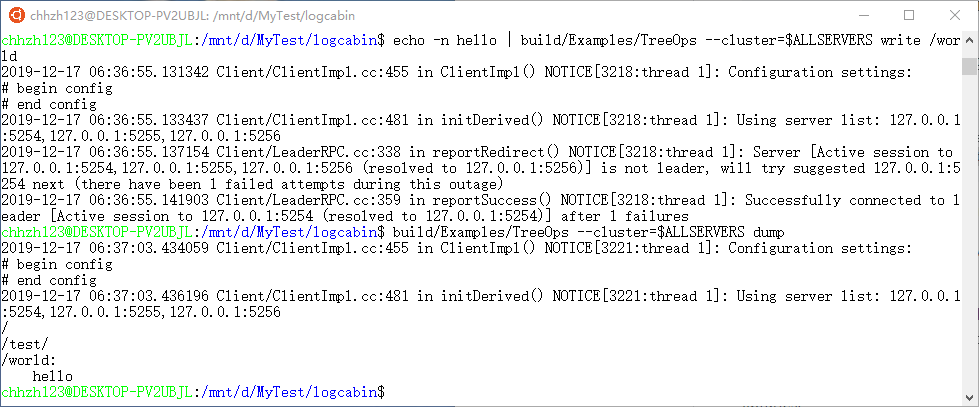
\includegraphics[width=\linewidth]{fig/mk_file.png}
\end{figure}

最后关闭其中一个服务器端,可以从下图看到其重新选举Leader的过程。
\begin{figure}[H]
\centering
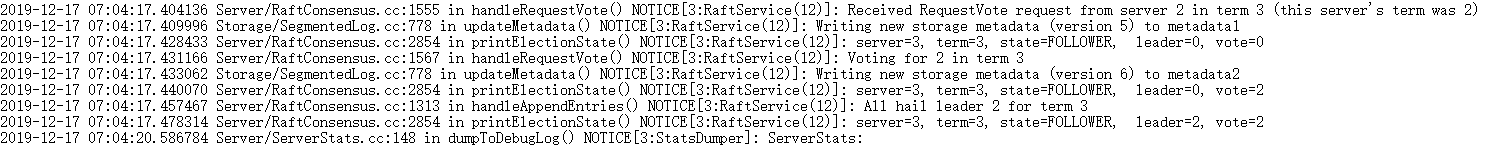
\includegraphics[width=\linewidth]{fig/re-election.png}
\end{figure}

从而通过此实验验证了raft共识协议的有效性,并且清晰地观察到其工作原理。
\end{answer}

\begin{thebibliography}{99}
\bibitem{bib:flooding} Flooding Consensus, \url{http://fileadmin.cs.lth.se/cs/Personal/Amr_Ergawy/dist-algos-slides/eigth-presentation.pdf}
\bibitem{bib:spanner} Google NewSQL Spanner, \url{https://en.wikipedia.org/wiki/Spanner_(database)}
\bibitem{bib:raft} RAFT Implementations, \url{https://raft.github.io/\#implementations}
\bibitem{bib:pbft} PBFT, \url{https://blockonomi.com/practical-byzantine-fault-tolerance/}
\bibitem{bib:bitcoin} Bitcoin, \url{https://blockonomi.com/bitcoin-mining-software/}
\end{thebibliography}

\end{document}